\documentclass[a4paper, 12pt]{article}

\usepackage{config}

\begin{document}
	\begin{titlepage}
		\begin{center}
			\begin{large}
				\textbf{Universidade Estadual de Campinas}\\\vspace{.5cm}
				\textbf{Faculdade de Engenharia Agrícola}\\\vspace{10.5cm}
			\end{large}
			\begin{large}
				\uppercase{\textbf{Compressão Uniaxial com Restrição e determinação do coeficiente de Poisson}}\\\vspace{4cm}
			\end{large}
		\end{center}
		\begin{large}
			\noindent\textbf{Nome:} \href{https://github.com/RenanSGuedes/576}{Renan da Silva Guedes}\\\\
			\noindent\textbf{RA:} 223979\\\vspace{4cm}
		\end{large}
		\begin{center}
			\begin{large}
				Campinas\\\vspace{.3cm}
				2020
			\end{large}
		\end{center}
	\end{titlepage}
	
	\newpage
	
	\section{Introdução}
	
	O ensaio a ser realizado consiste na compressão uniaxial com restrição de corpos de prova (CP) de batata inglesa, dando continuidade ao primeiro experimento. Dessa forma, a partir das repetições realizadas também é visada a determinação do coeficiente de Poisson ($\nu$) do material estudado.
	
	\section{Objetivos}
	
	Determinação do coeficiente de Poisson ($\nu$)
	
	\section{Materiais e Métodos}
	
	Para a realização do experimento foi feito uso das batatas, cortador cilíndrico para as mesmas, cilindro vazado para a inserção dos CPs, paquímetro digital, Máquina Universal de Ensaios e \textit{software} para aquisição de dados. 
	
	Dessa forma, após seguir os procedimentos iniciais apresentados na figura \ref{diagram} e realizar cinco repetições de compressão dos corpos de provas nas condições de restrição vistas no cilindro vazado, foi obtido o gráfico mostrado na Figura \ref{graph}.
	
	Feito isso, foi após linearizar os trechos pertinentes de cada curva, foi encontrado o parâmetro (M) a ser substituído na equação \eqref{main_eq}. Em seguida, ao fazer a interpolação dos valores de módulo de elasticidade (E) para a velocidade de \SI{1}{\milli\meter/\second} aplicada nas 5 repetições chegou-se no valor de $\textrm{E}=\SI{3.64}{\giga\pascal}$. Sendo $\textrm{M}=\SI{5.14}{\giga\pascal}$ (coeficiente angular médio dos trechos linearizados para as cinco curvas da Figura \ref{graph}), chegou-se que o coeficiente de Poisson é de $0.32$.
	
	\section{Resultados e Discussão}
	\section{Conclusão}
	
	\section{Anexos}
	
	\import{tables/}{data}
	
	\begin{figure}
		\label{diagram}
		\centering
		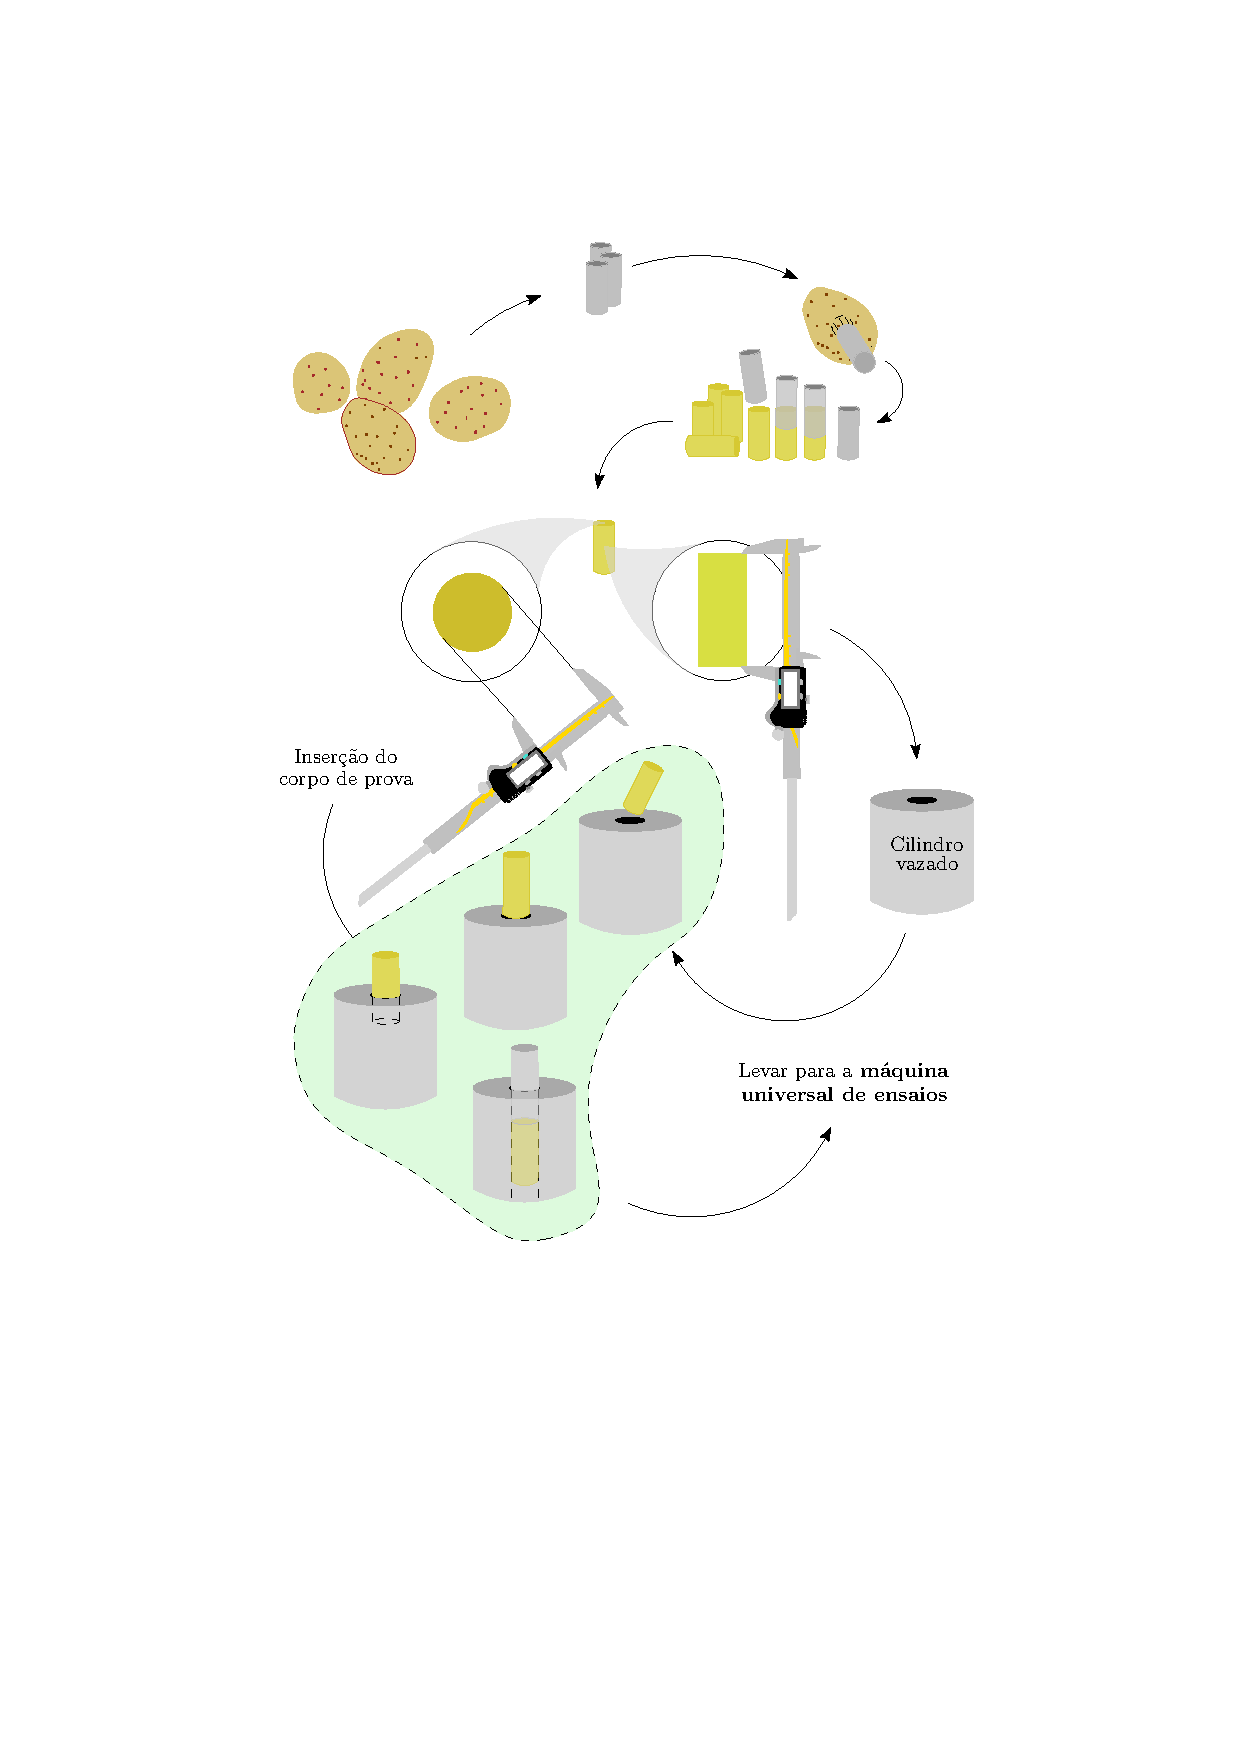
\includegraphics[scale=1.1]{images/diagram}
		\caption{Procedimentos adotados na elaboração de cada CP de batata inglesa. Após cortar a mesma no formato cilíndrico deve ser feita sua inserção no cilindro vazado seguido do cilindro que vai comprimir o CP por ação da Máquina Universal de Ensaios.}
	\end{figure}

	\begin{figure}
		\label{graph}
		\centering
		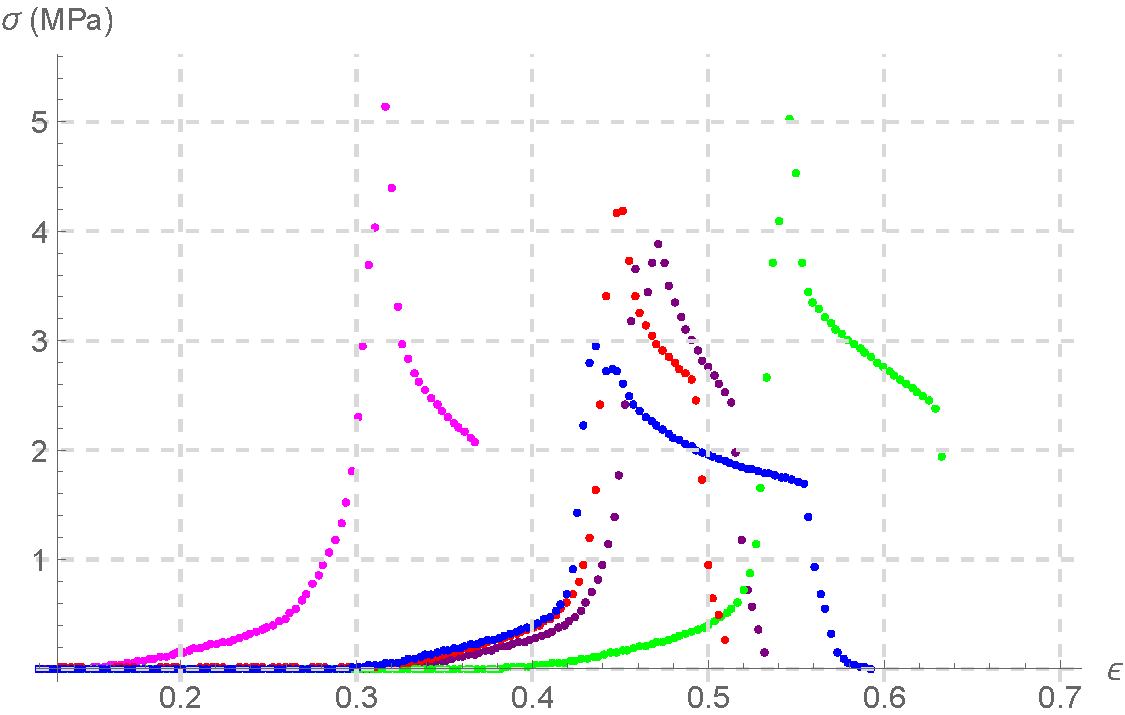
\includegraphics[scale=.6]{images/graph}
		\caption{Gráfico tensão \textit{versus} deformação para os corpos de prova sob compressão à velocidade de \SI{1}{\milli\meter/\second}.}
	\end{figure}
	
	
	\subsection{Equações}
		
	\begin{equation}\label{main_eq}
		\textrm{M}=\dfrac{\textrm{E}}{(1-\nu)}\cdot\dfrac{(1-\nu)}{(1+\nu)}
	\end{equation}
\end{document}